\chapter{程式碼說明}
\renewcommand{\baselinestretch}{10.0} %設定行距
\pagenumbering{arabic} %設定頁號阿拉伯數字
\setcounter{page}{5}  %設定頁數
\fontsize{14pt}{2.5pt}\sectionef

\section{控制機器人程式}
\begin{figure}[hbt!]
\begin{center}
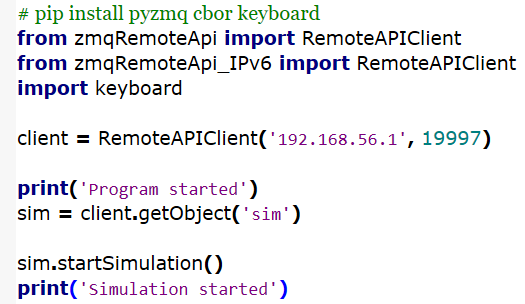
\includegraphics[height=5cm]{bubbleRob code 1}
\caption{\Large 控制機器人程式之一}\label{控制機器人程式之一}
\end{center}
\end{figure} 
使用 pip install pyzmq cbor keyboard 安裝了所需的套件,其中 pyzmq 是用於建立 ZeroMQ 連線,cbor 是用於將資料序列化和反序列化,keyboard 是用於操控鍵盤事件,使用 from zmqRemoteApi import RemoteAPIClient 和 from zmqRemoteApi_IPv6 import RemoteAPIClient 導入了用於建立與 CoppeliaSim 之間通訊的 Remote API 相關程式庫。這些程式庫提供了與 CoppeliaSim 的介面,使得可以通過程式碼控制仿真場景和物件,建立了一個 RemoteAPIClient 物件 client,並將 192.168.56.1 和 19997 分別作為 CoppeliaSim 的 IP 地址和連接埠進行初始化。這樣就建立了與 CoppeliaSim 的連線,使用 client.getObject('sim') 獲取了 CoppeliaSim 中的 sim 物件,該物件代表了整個仿真環境。透過這個物件,可以執行相關的仿真操作,再來透過  sim.startSimulation() 開始模擬。\\[6pt]
\begin{figure}[hbt!]
\begin{center}
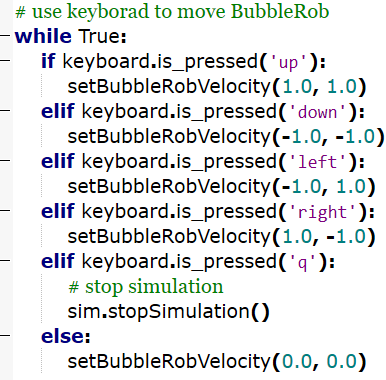
\includegraphics[height=8cm]{bubbleRob code 2}
\caption{\Large 控制機器人程式之二}\label{控制機器人程式之二}
\end{center}
\end{figure} 
這段程式碼是一個無窮迴圈,用於持續監聽鍵盤事件並根據按鍵的狀態來控制機器人的運動,如果按下 'up' 鍵,則呼叫 setBubbleRobVelocity(1.0, 1.0),將機器人的速度設定為正向。如果按下 'down' 鍵,則呼叫 setBubbleRobVelocity(-1.0, -1.0),將機器人的速度設定為反向。如果按下 'left' 鍵,則呼叫 setBubbleRobVelocity(-1.0, 1.0),將機器人的速度設定為左轉。如果按下 'right' 鍵,則呼叫 setBubbleRobVelocity(1.0, -1.0),將機器人的速度設定為右轉。如果按下 'q' 鍵,則停止仿真。若沒有按下上述任何按鍵,則呼叫 setBubbleRobVelocity(0.0, 0.0),將機器人的速度設定為零,即停止移動。\\[6pt]
\renewcommand{\baselinestretch}{0.5} %設定行距